\documentclass[11pt,a4paper]{article}
\usepackage{polski}
\usepackage[utf8]{inputenc}
\usepackage[colorlinks=true,linkcolor=black,urlcolor=blue,citecolor=RoyalBlue]{hyperref}
\usepackage[usenames,dvipsnames]{color}
\usepackage{alltt}
\usepackage{booktabs} % eleganckie tabelki
\usepackage{graphicx}
\usepackage{hyperref}

\newcounter{liczp}
\newenvironment{example}{\refstepcounter{liczp}{\noindent
{\bf Przykład~\theliczp:}\,}}


\addtolength{\textwidth}{4cm}
\addtolength{\hoffset}{-2cm}
\addtolength{\textheight}{4cm}
\addtolength{\voffset}{-2cm}
\date {\today}
\author {Aleksy Barcz}
\title{Implementacja algorytmu JOR w technologii CUDA\\sprawozdanie}
\begin{document}
\maketitle

\section{Algorytm JOR}
Algorytm zaimplementowano zgodnie ze wzorem:
\begin{equation}
x_j^{i+1} \; = \; (1-\alpha) x_j^i \, + \, \frac{\alpha}
{A_{jj}} \, \left(b_j - \sum_{k\not=j} A_{jk}
x_k^i\right)
\end{equation}
(\url{http://staffweb.cms.gre.ac.uk/~ct02/research/thesis/node36.html})\\

\section{Narzędzia}
Projekt wykonano przy użyciu gcc w wersji 4.9.1 oraz Nvidia CUDA toolkit w wersji 6.0.37 na systemie Debian testing. Eksperymenty przeprowadzono na komputerze z 4-rdzeniowym procesorem i5-4670K CPU @ 3.40GHz i kartą graficzną Nvidia Quadro 4000, wspierającą architekturę CUDA w wersji 2.0, zapewniającą m.in. dobre wsparcie dla typu double, w przeciwieństwie do mocno ograniczonej architektury 1.3.

\section{Zastosowane metody zrównoleglania / wektoryzacji}
W projekcie porównano działanie algorytmu dla następujących implemenetacji:
\begin{enumerate}
	\item algorytm bez optymalizacji (ozn. 'CPU'),
	\item algorytm z wektoryzacją wewnętrznej pętli (OpenMP, ozn. 'SIMD'),
	\item algorytm ze zrównolegleniem wątkowym obu pętli (OpenMP, ozn. 'OMP'),
	\item algorytm wykonujący całość obliczeń macierzowych na karcie graficznej (ozn. 'CUDA').
\end{enumerate}

\section{Dane wejściowe}
W każdym przypadku, dzięki zastosowaniu tego samego ziarna generatora liczb losowych, przetwarzane było te same dziesięć macierzy określonego rozmiaru, dla rozmiarów (ilość wierszy kwadratowej macierzy A): 128, 256, 512, 1024, 2048, 4096, 8192. Eksperymenty przeprowadzono dla obliczeń dla dwóch rodzajów elementów macierzy: double oraz float. Macierze generowano, losując wartości elementów z zakresu $[-5, 5]$, a następnie zapewniając że każdy element głównej przekątnej macierzy $A$ będzie większy o losową wartość od sumy pozostałych elementów wiersza (aby dla macierzy $A$ zachodziła bezwzględna dominacja wierszowa głównej przekątnej).

\section{Konfiguracja algorytmu}
Dla algorytmu JOR dobrano eksperymentalnie wartość $\alpha$ równą $0.9$, jako dającą niewielką liczbę iteracji algorytmu i mniejszą od $1.0$, co jest istotne dla dowodu o zbieżności algorytmu. Jako kryterium stopu wybrano minimalną różnicę $min_j(abs(x_j^{i+1} - x_j^{i}))$ o wartości $10^{-8}$ dla typu double i $10^{-6}$ dla float - mniejsze wartości powodowały brak zbieżności algorytmu dla typu float.

\section{Implementacja w CUDA}
W CUDA zaimplementowano trzy metody: mnożenie macierzy, obliczenie nowej wartości $x$ oraz obliczenie różnicy  $min_j(abs(x_j^{i+1} - x_j^{i}))$. Dzięki przeniesieniu tych wszystkich operacji na kartę graficzną, kopiowanie macierzy między pamięcią komputera a kartą graficzną odbywa się tylko raz przed rozpoczęciem obliczeń oraz na sam koniec, w celu pobrania końcowej wartości $x$. W międzyczasie do pamięci komputera przekazywany jest tylko jeden skalar - różnica między macierzami $x$ po kolejnej iteracji algorytmu. Z tych trzech operacji, znaczącą większość czasu (ok. 90\%) zajmuje mnożenie macierzy $A$ i $x$, w związku z tym główny wysiłek polegał na optymalnej implementacji tego mnożenia. Po eksperymentach z m.in. pamięcią \emph{shared memory}, ostatecznie zaimplementowano najszybszą w tym przypadku metodę - opartą o \emph{memory coalescence}(\url{http://www.johnhawthorn.com/2012/03/squeezing-performance-from-cuda/}). W trakcie mnożenia poszczególne wątki w ten sposób indeksują macierze $A$ i $x$ aby odczyty z pamięci globalnej GPU były zbijane w bloki, redukując w ten sposób znacznie ilość odczytów. Zadanie podzielono tak, aby za obliczenie jednego elementu wynikowej macierzy odpowiadał cały jeden blok rdzeni. Każdy blok podzielono na 128 wątków (wartość dobrana eksperymentalnie jako optymalna dla wielkości macierzy od 2048 do 8192), każdy z wątków przetwarza tylko część wiersza macierzy $A$. Końcową wartość elementu wynikającego z działania całego bloku oblicza się wykonując redukcję w obrębie bloku metodą \emph{reversed loop with threadID-based indexing}(\url{http://developer.download.nvidia.com/assets/cuda/files/reduction.pdf}), która okazała się najszybsza (rozwinięcie ostatnich kroków pętli redukcji okazało się mniej efektywne). Na sam koniec wątek o numerze 0 przepisuje zredukowaną sumę do odpowiedniego elementu macierzy wynikowej.

Dodatkowo, dla typu danych float umieszczono macierz A, jako stałą dla wszystkich iteracji algorytmu, w pamięci tekstur, co minimalnie przyspieszyło obliczenia. Użycie pamięci tekstur nie wpłynęło na wynikowy RMSE modelu.

\section{Wyniki - omówienie}
Pod względem jakości wyniku (najmniejsze RSME) znacząco lepszy okazał się algorytm zaimplementowany przy użyciu typu double. Jeśli chodzi o czas obliczeń i możliwości przyspieszania lepszy okazał się algorytm zaimplementowany przy użyciu typu float.

Dla obu typów widać interesujące zależności od rozmiaru macierzy. Dla bardzo małych macierzy najbardziej opłaca się wykorzystywać wektoryzację CPU. Od rozmiaru 256 wektoryzacja wątkowa na CPU zaczyna dawać lepsze efekty niż wektoryzacja CPU. Z kolei implementacja w CUDA zaczyna wygrywać dopiero przy dużych rozmiarach macierzy - od 2048 dla typu double i od 4096 dla typu float. Jednocześnie można zauważyć, że nawet dla niewielkich macierzy opłaca się optymalizacja na CPU, tymczasem narzut związany z użyciem GPU powoduje, że dla niewielkich macierzy użycie GPU powoduje wydłużenie czasu obliczeń w stosunku do algorytmu sekwencyjnego.

Na wykresach zaprezentowano średnie czasy obliczeń dla poszczególnych rozmiarów macierzy. Użyte kolory to: czerwony-CPU, zielony-SIMD, niebieski-OMP, magenta-CUDA.

\newpage
\section{Wyniki - double}

\begin{table}[h!]
\begin{center}
\begin{tabular}{lllll}
\toprule
rozmiar macierzy & \textcolor{red}{CPU} & \textcolor{green}{SIMD} & \textcolor{blue}{OMP} & \textcolor{magenta}{CUDA} \\
\midrule
128 &  0.00014 (0.00000) &  0.00010 (0.00000) &  0.00012 (0.00007) &  0.00218 (0.01331) \\
256 &  0.00056 (0.00007) &  0.00034 (0.00004) &  0.00029 (0.00007) &  0.00266 (0.01349) \\
512 &  0.00224 (0.00000) &  0.00124 (0.00002) &  0.00079 (0.00003) &  0.00359 (0.01321) \\
1024 &  0.00930 (0.00006) &  0.00540 (0.00007) &  0.00357 (0.00006) &  0.00662 (0.01357) \\
2048 &  0.03677 (0.00011) &  0.02266 (0.00011) &  0.01831 (0.00032) &  0.01660 (0.01314) \\
4096 &  0.14819 (0.00014) &  0.09336 (0.00024) &  0.07506 (0.00025) &  0.05593 (0.01421) \\
8192 &  0.59742 (0.00129) &  0.37804 (0.00046) &  0.31137 (0.00061) &  0.21477 (0.01569) \\
\bottomrule
\end{tabular}
\caption{Średni czas działania [s] (odchylenie std.)}
\end{center}
\end{table}

\begin{figure}[h!]
\begin{center}
	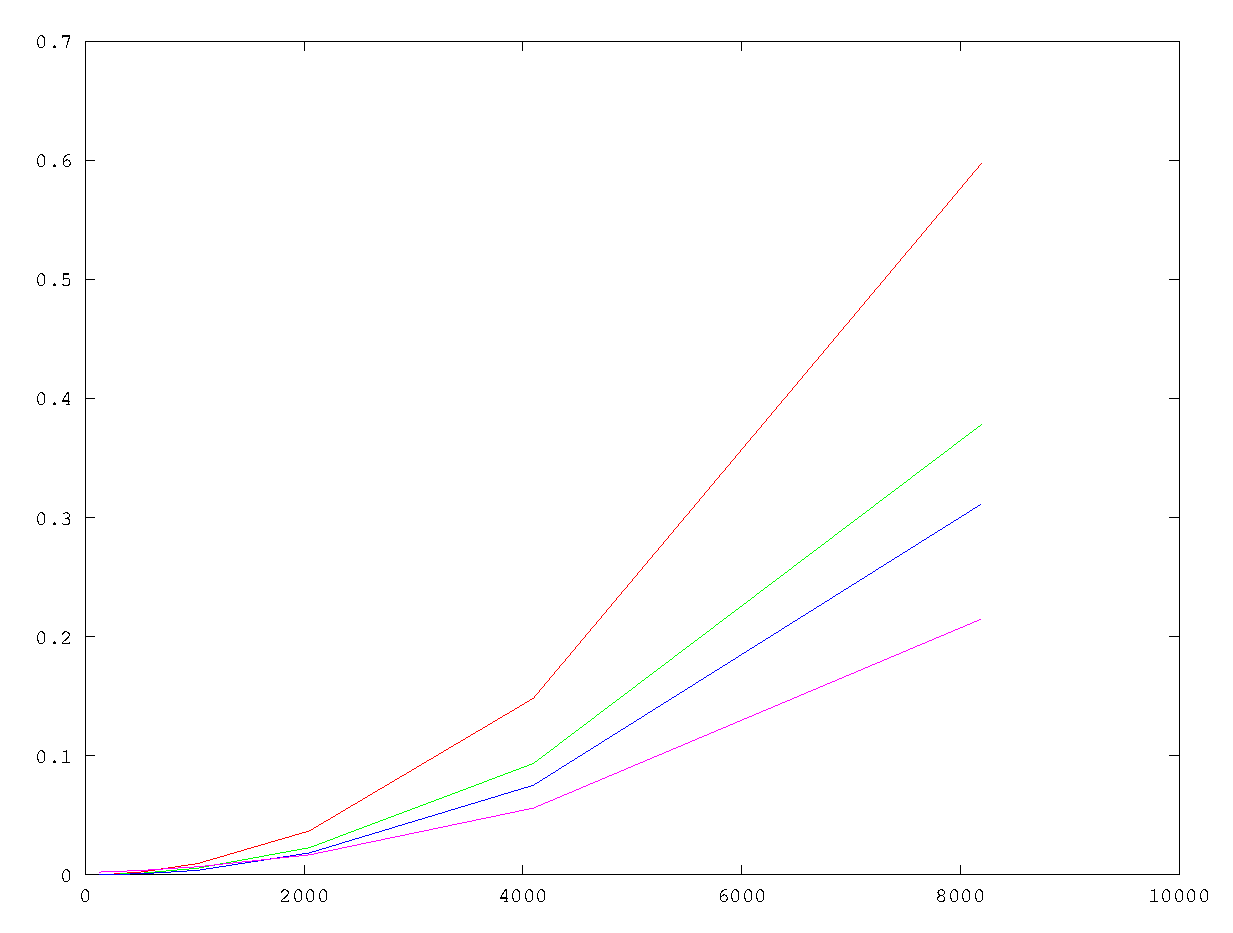
\includegraphics[scale=0.45]{double_time}
	\caption{Średni czas działania [s]}
	\label{fig:double_time}
\end{center}
\end{figure}

\begin{figure}[h!]
\begin{center}
	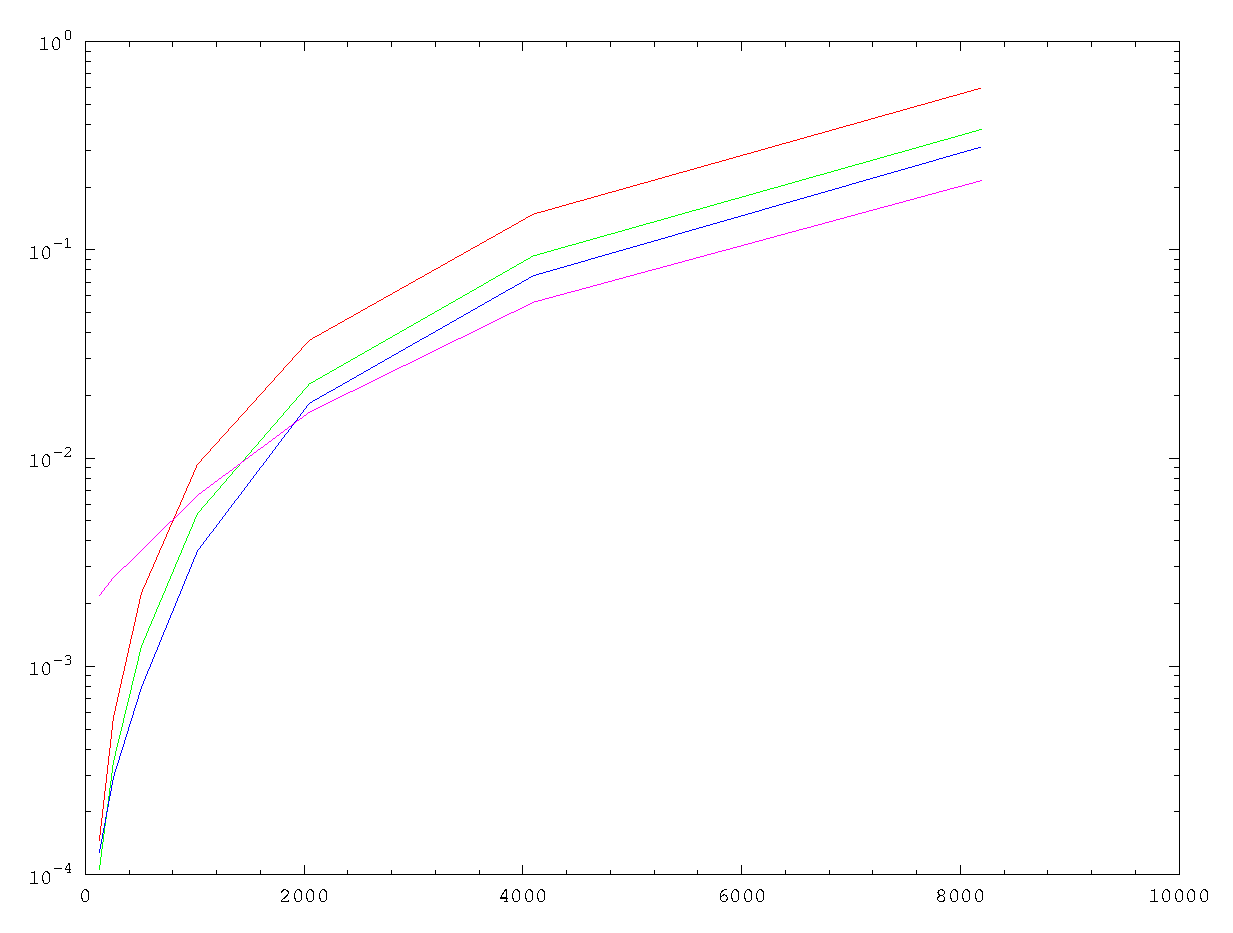
\includegraphics[scale=0.45]{double_time_log}
	\caption{Logarytm ze średniego czasu działania}
	\label{fig:double_time_log}
\end{center}
\end{figure}

\newpage

\begin{table}[h!]
\begin{center}
\begin{tabular}{llll}
\toprule
rozmiar macierzy & SIMD & OMP & CUDA \\
\midrule
128 & 1.37 & 1.14 & 0.06 \\
256 & 1.63 & 1.93 & 0.21 \\
512 & 1.80 & 2.83 & 0.62 \\
1024 & 1.72 & 2.60 & 1.40 \\
2048 & 1.62 & 2.00 & 2.21 \\
4096 & 1.58 & 1.97 & 2.64 \\
8192 & 1.58 & 1.91 & 2.78 \\
\bottomrule
\end{tabular}
\caption{Współczynnik przyspieszenia}
\end{center}
\end{table}

\begin{table}[h!]
\begin{center}
\begin{tabular}{lllll}
\toprule
r.m. & CPU & SIMD & OMP & CUDA \\
\midrule
128 &  0.0000009 (0.0000005) &  0.0000009 (0.0000005) &  0.0000009 (0.0000005) &  0.0000013 (0.0000027) \\
256 &  0.0000062 (0.0000105) &  0.0000062 (0.0000105) &  0.0000062 (0.0000105) &  0.0000056 (0.0000092) \\
512 &  0.0000111 (0.0000021) &  0.0000111 (0.0000021) &  0.0000111 (0.0000021) &  0.0000111 (0.0000028) \\
1024 &  0.0000175 (0.0000019) &  0.0000175 (0.0000019) &  0.0000175 (0.0000019) &  0.0000181 (0.0000023) \\
2048 &  0.0000334 (0.0000027) &  0.0000334 (0.0000027) &  0.0000334 (0.0000027) &  0.0000334 (0.0000022) \\
4096 &  0.0000704 (0.0000027) &  0.0000704 (0.0000027) &  0.0000704 (0.0000027) &  0.0000714 (0.0000022) \\
8192 &  0.0001687 (0.0000059) &  0.0001687 (0.0000059) &  0.0001687 (0.0000059) &  0.0001683 (0.0000045) \\
\bottomrule
\end{tabular}
\caption{RMSE (odchylenie std.)}
\end{center}
\end{table}

\newpage
\section{Wyniki - float}

\begin{table}[h!]
\begin{center}
\begin{tabular}{lllll}
\toprule
rozmiar macierzy & \textcolor{red}{CPU} & \textcolor{green}{SIMD} & \textcolor{blue}{OMP} & \textcolor{magenta}{CUDA} \\
\midrule
128 &  0.00000 (0.00000) &  0.00000 (0.00000) &  0.00009 (0.00092) &  0.00253 (0.01482) \\
256 &  0.00029 (0.00141) &  0.00009 (0.00092) &  0.00019 (0.00123) &  0.00234 (0.01297) \\
512 &  0.00214 (0.00123) &  0.00078 (0.00123) &  0.00078 (0.00123) &  0.00302 (0.01335) \\
1024 &  0.00820 (0.00204) &  0.00214 (0.00123) &  0.00253 (0.00151) &  0.00458 (0.01273) \\
2048 &  0.03193 (0.00535) &  0.00976 (0.00138) &  0.00937 (0.00151) &  0.00966 (0.01356) \\
4096 &  0.13046 (0.01944) &  0.03818 (0.00092) &  0.03681 (0.00618) &  0.02714 (0.01365) \\
8192 &  0.53232 (0.05056) &  0.15976 (0.02223) &  0.15029 (0.01438) &  0.09433 (0.01482) \\
\bottomrule
\end{tabular}
\caption{Średni czas działania [s] (odchylenie std.)}
\end{center}
\end{table}

\begin{figure}[h!]
\begin{center}
	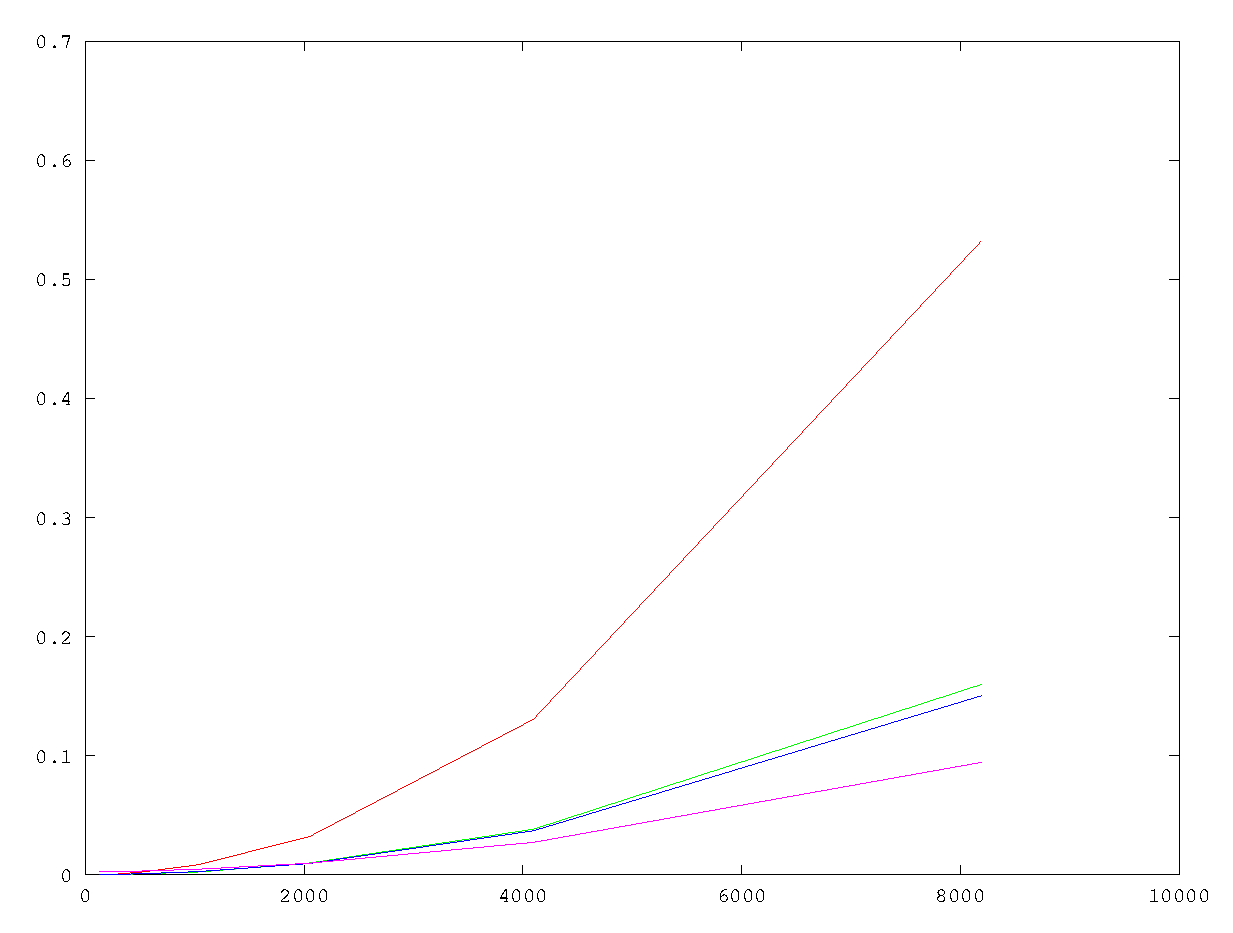
\includegraphics[scale=0.45]{float_time}
	\caption{Średni czas działania [s]}
	\label{fig:float_time}
\end{center}
\end{figure}

\begin{figure}[h!]
\begin{center}
	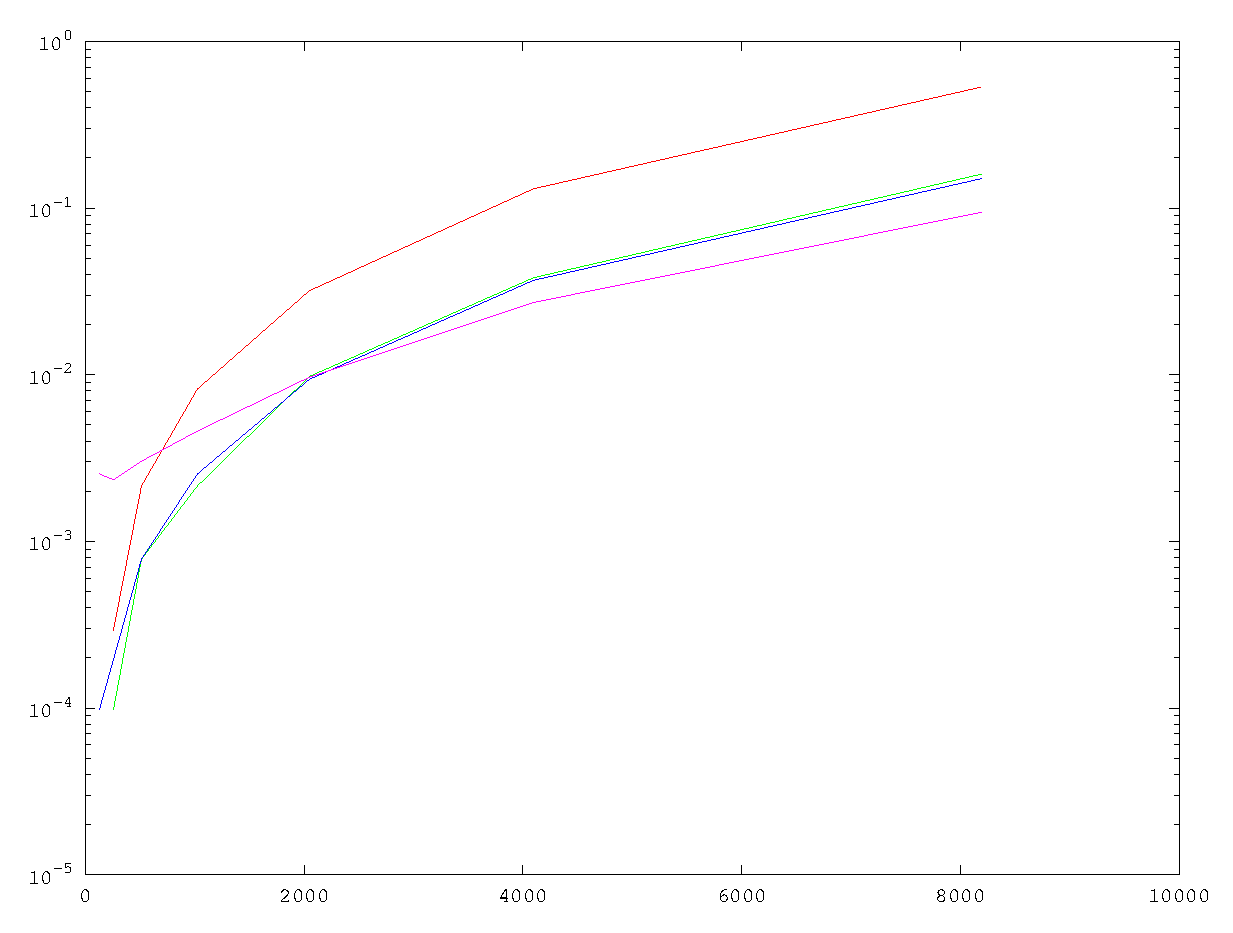
\includegraphics[scale=0.45]{float_time_log}
	\caption{Logarytm ze średniego czasu działania}
	\label{fig:float_time_log}
\end{center}
\end{figure}

\newpage


\begin{table}[h!]
\begin{center}
\begin{tabular}{llll}
\toprule
rozmiar macierzy & SIMD & OMP & CUDA \\
\midrule
128 & ? & \textless 1.0 & \textless 1.0 \\
256 & 2.99 & 1.50 & 0.12 \\
512 & 2.75 & 2.75 & 0.70 \\
1024 & 3.81 & 3.23 & 1.78 \\
2048 & 3.27 & 3.40 & 3.30 \\
4096 & 3.41 & 3.54 & 4.80 \\
8192 & 3.33 & 3.54 & 5.64 \\
\bottomrule
\end{tabular}
\caption{Współczynnik przyspieszenia}
\end{center}
\end{table}

\begin{table}[h!]
\begin{center}
\begin{tabular}{lllll}
\toprule
r.m. & CPU & SIMD & OMP & CUDA \\
\midrule
128 &  0.00109 (0.00030) &  0.00420 (0.00102) &  0.00109 (0.00030) &  0.00463 (0.00119) \\
256 &  0.00311 (0.00108) &  0.01552 (0.00383) &  0.00311 (0.00108) &  0.01824 (0.00522) \\
512 &  0.00795 (0.00236) &  0.05856 (0.01221) &  0.00795 (0.00236) &  0.06739 (0.01377) \\
1024 &  0.02170 (0.00439) &  0.23708 (0.02600) &  0.02170 (0.00439) &  0.26990 (0.03218) \\
2048 &  0.06414 (0.01342) &  0.89628 (0.05912) &  0.06414 (0.01342) &  1.02248 (0.10288) \\
4096 &  0.17414 (0.02825) &  3.55114 (0.20252) &  0.17414 (0.02825) &  4.05389 (0.14852) \\
8192 &  0.47507 (0.04823) &  14.0111 (0.38742) &  0.47507 (0.04823) &  16.1029 (0.55284) \\
\bottomrule
\end{tabular}
\caption{RMSE (odchylenie std.)}
\end{center}
\end{table}

\end{document}
